\documentclass[aspectratio=169]{beamer}
\usetheme[block=fill]{metropolis}
\usepackage{tikz}
\usetikzlibrary{shapes.geometric, arrows.meta, positioning, calc}

\title{Building a Reproducible Scholarly Search Toolkit}
\subtitle{Episode 6: Clusters \& Duplicate Aggregation}
\author{Scholar Search Kit}
\date{}

\begin{document}

\begin{frame}[plain]
  \titlepage
\end{frame}

\begin{frame}{Episode Goal}
  \begin{alertblock}{The Goal}
    Create a \texttt{DocumentCluster} model to hold exact-duplicate documents without destroying data.
  \end{alertblock}
  \vspace{0.5cm}
  If OpenAlex and arXiv both return the exact same paper, we shouldn't arbitrarily delete one. We must cluster them together and retain the provenance of both.
\end{frame}

\begin{frame}{Non-Destructive Merging}
  \begin{center}
  \resizebox{0.6\linewidth}{!}{
  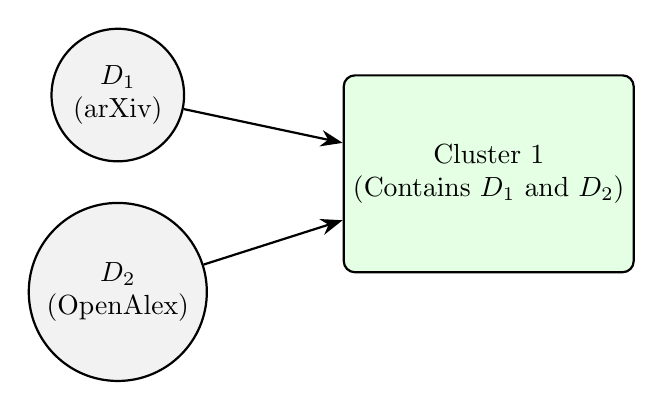
\begin{tikzpicture}[
      node distance=1.5cm and 2cm,
      doc/.style={circle, draw, thick, minimum size=1.5cm, align=center, fill=black!5},
      cluster/.style={rectangle, draw, thick, rounded corners, minimum width=3.5cm, minimum height=2.5cm, align=center, fill=green!10},
      arrow/.style={-{Stealth[scale=1.2]}, thick}
    ]
    
    \node[doc] (d1) {$D_1$\\(arXiv)};
    \node[doc, below=0.5cm of d1] (d2) {$D_2$\\(OpenAlex)};
    
    \node[cluster, right=of d1, yshift=-1cm] (c1) {Cluster 1\\(Contains $D_1$ and $D_2$)};
    
    \draw[arrow] (d1) -- (c1);
    \draw[arrow] (d2) -- (c1);
  \end{tikzpicture}
  }
  \end{center}
\end{frame}

\begin{frame}{The \texttt{DocumentCluster} Model}
  \begin{block}{Holding the Bag}
    A cluster is effectively a list of documents that we are confident are the same entity.
  \end{block}
  
  \begin{itemize}
      \item \texttt{documents}: A List of \texttt{Document} objects.
      \item \texttt{match\_confidence}: E.g., \texttt{1.0} for exact DOI matches, \texttt{0.95} for fuzzy title matches.
      \item \texttt{canonical\_document}: Property to extract the "best" version for export.
  \end{itemize}
\end{frame}

\begin{frame}{Implementation: Confidence Metrics}
  \begin{block}{Why Confidence Matters}
    In an SLR, merging two distinct papers by accident is a fatal flaw.
  \end{block}
  
  \begin{itemize}
      \item We explicitly track the confidence level of a cluster.
      \item If confidence is low, the AI Harness can flag it for human review.
  \end{itemize}
\end{frame}

\begin{frame}{Verification}
  \begin{alertblock}{Success Criteria}
    \begin{itemize}
        \item A cluster can be initialized with multiple documents.
        \item The \texttt{canonical\_document} property successfully picks the document with the most populated fields.
    \end{itemize}
  \end{alertblock}
\end{frame}

\end{document}
